\begin{figure}[htbp]
\centering
\begin{tikzpicture}[schema base]
\node[schema titolo] at (0,0.3) {Dimensione del ritaglio e informazione visibile};
\node[schema etichetta] at (3.25,-0.6) {\textbf{Ingombro sulla pagina 8}};
\path[draw=schemaGrigio,fill=schemaGrigio!4] (0,-1.15) rectangle (6.5,-6.025);
\node[schema nota,text width=5.5cm] at (3.25,-2.15)
  {Pagina: $2600\times1950$\\Sistema di coordinate del bundle};
\path[draw=schemaOcra,fill=schemaCartaGialla,line width=1.2pt]
  ({1433/400},{-1.15-1052/400}) rectangle ({1761/400},{-1.15-1324/400});
\draw[schemaGrigio,line width=0.65pt]
  ({1433/400},-3.5) -- ({1761/400},-3.5);
\foreach \ascissa in {1433,1761} {
  \draw[schemaGrigio,line width=0.65pt] ({\ascissa/400},-3.42) -- ({\ascissa/400},-3.58);
}
\node[schema nota,font=\schemafont\footnotesize] at ({1597/400},-3.18) {328 px};
\draw[schemaGrigio,line width=0.65pt]
  (3.3,{-1.15-1052/400}) -- (3.3,{-1.15-1324/400});
\foreach \ordinata in {1052,1324} {
  \draw[schemaGrigio,line width=0.65pt] (3.22,{-1.15-\ordinata/400}) -- (3.38,{-1.15-\ordinata/400});
}
\node[schema nota,font=\schemafont\footnotesize,anchor=east] at (3.08,{-1.15-1188/400}) {272 px};
\node[schema nota,text width=5.7cm] at (3.25,-5.35)
  {Solo l'ingombro è rappresentato:\\non è il rendering della pagina.};
\node[schema etichetta] at (11.5,-0.6) {\textbf{Lo stesso ritaglio, ingrandito}};
\node[inner sep=0] (crop) at (11.5,-3.45)
  {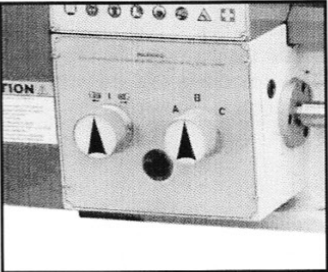
\includegraphics[width=4.6cm]{figure/asset/v4/paddle-image-0008-0003.png}};
\draw[schemaOcra,line width=1pt,line cap=round,line join=round]
  ([xshift=-3pt,yshift=-9pt]crop.north west) -- ([xshift=-3pt,yshift=3pt]crop.north west) -- ([xshift=9pt,yshift=3pt]crop.north west)
  ([xshift=-9pt,yshift=3pt]crop.north east) -- ([xshift=3pt,yshift=3pt]crop.north east) -- ([xshift=3pt,yshift=-9pt]crop.north east)
  ([xshift=-3pt,yshift=9pt]crop.south west) -- ([xshift=-3pt,yshift=-3pt]crop.south west) -- ([xshift=9pt,yshift=-3pt]crop.south west)
  ([xshift=-9pt,yshift=-3pt]crop.south east) -- ([xshift=3pt,yshift=-3pt]crop.south east) -- ([xshift=3pt,yshift=9pt]crop.south east);
\draw[schemaOcra,line width=1.1pt] (7.4,-2.65) circle (0.28);
\draw[schemaOcra,line width=1.8pt,line cap=round] (7.6,-2.85) -- (7.92,-3.17);
\draw[schema freccia,draw=schemaOcra] ({1761/400},{-1.15-1188/400}) -- (7.4,{-1.15-1188/400}) |- (crop.west);
\node[schema nota] at (11.5,-5.85) {Ritaglio: $328\times272$ pixel};
\node[schema blocco,text width=6.2cm,minimum height=1.9cm] at (3.5,-7.5)
  {\textbf{Regola geometrica}\\$\rho=\dfrac{328\cdot272}{2600\cdot1950}\simeq1{,}76\%$\\Inferiore alla soglia del $2\%$};
\node[schema esterno,text width=6.2cm,minimum height=1.9cm] at (11.5,-7.5)
  {\textbf{Conseguenza osservata}\\Nessuna chiamata al VLM\\Asset conservato, escluso dall'uso\\Comandi e simboli restano visibili};
\end{tikzpicture}
\caption{Filtro geometrico su \texttt{paddle-image-0008-0003}: a sinistra la posizione registrata in \texttt{manual.json}, a destra il ritaglio originale. L'immagine è esclusa prima della generazione, non per un errore del modello.}
\label{fig:crop-escluso-wm250}
\end{figure}